\documentclass[
    table,
    12pt,
    oneside,
    a4paper,
    italian
]{book}

\PassOptionsToPackage{dvipsnames}{xcolor} % colori PDF/A

\usepackage{colorprofiles}
% PDF/A
% validate in https://www.pdf-online.com/osa/validate.aspx
\usepackage[a-1a,mathxmp]{pdfx}[2018/12/22]
\usepackage[T1]{fontenc}
\usepackage[utf8]{inputenc}
\usepackage[italian]{babel}
\usepackage{bookmark}
\usepackage{caption}
\usepackage{comment}
\usepackage{chngpage, calc} % centra il frontespizio
\usepackage{emptypage} % pagine vuote senza testatina e piede di pagina
\usepackage{epigraph} % per epigrafi
\usepackage{indentfirst} % rientra il primo paragrafo di ogni sezione
\usepackage{graphicx} % immagini
\usepackage[pdfa]{hyperref} % collegamenti ipertestuali
\usepackage{mparhack,relsize}  % finezze tipografiche
\usepackage{nameref} % visualizza nome dei riferimenti
\usepackage[font=small]{quoting} % citazioni
\usepackage{subfig} % sottofigure, sottotabelle
\usepackage[italian]{varioref} % riferimenti completi della pagina
\usepackage{longtable} % tabelle su più pagine
\usepackage[toc, acronym, automake]{glossaries}
\usepackage[backend=biber, style=verbose-ibid, hyperref, backref]{biblatex}
\usepackage{lmodern}
\usepackage[top=2.75cm, bottom=2.75cm, right=3cm, left=3cm]{geometry} % 1in+17pt+0.6cm
%\usepackage[top=2.75cm, bottom=2.75cm, right=3cm, left=3.75cm]{geometry} % 1in+17pt+0.6cm
\usepackage{fancyhdr}
\usepackage{lipsum}
\usepackage{setspace}
\usepackage{titlesec}
\usepackage{minted} % https://it.overleaf.com/learn/latex/Code_Highlighting_with_minted
\usepackage{xcolor}
\usepackage{csquotes} % gestisce automaticamente i caratteri (")
\usepackage{etoolbox}
\usepackage{dirtree}
% Load variables
\newcommand{\myUni}{Università degli Studi di Padova}
\newcommand{\myDepartment}{Dipartimento di Matematica ``Tullio Levi-Civita''}
\newcommand{\myFaculty}{Corso di Laurea in Informatica}
\newcommand{\myTitle}{Lorem ipsum dolor sit amet, consectetur adipisci elit.}
\newcommand{\myDegree}{Tesi di Laurea Triennale}
\newcommand{\profTitle}{Prof.}
\newcommand{\myProf}{Cognome Nome}
\newcommand{\graduateTitle}{Laureando}
\newcommand{\myName}{Bobirica Andrei Cristian}
\newcommand{\myStudentID}{1224449}
\newcommand{\myAA}{2023-2024}
\newcommand{\myLocation}{Padova}
\newcommand{\myTime}{Luglio 2024}
% Glossary
\newacronym{ddc}{DDC}{Data Driven Cooking}
\newglossaryentry{ddcg}{
    name={DDC},
    text={Data Driven Cooking},
    sort=ddc,
    description={Una piattaforma di cucina intelligente che utilizza i dati per ottimizzare e migliorare i processi di cottura. DDC fornisce funzionalità avanzate per i proprietari di forni, consentendo loro di monitorare e controllare i dispositivi in modo efficiente}
}

\newacronym{rtk}{RTK}{Redux Toolkit}
\newglossaryentry{rtkg}{
    name={RTK},
    text={Redux Toolkit},
    sort=rtk,
    description={Un toolkit per Redux che semplifica la scrittura della logica Redux e automatizza configurazioni complesse. RTK è stato utilizzato per gestire lo stato globale dell'applicazione in modo efficiente e strutturato}
}

\newacronym{cicd}{CI/CD}{continuous integration and continuous delivery}
\newglossaryentry{cicdg}{
    name={CI/CD},
    text={CI/CD},
    sort=cicd,
    description={Integrazione continua e consegna continua. L'integrazione continua (CI) è una pratica di sviluppo software in cui i membri del team integrano il loro lavoro frequentemente, con verifiche automatizzate per rilevare errori rapidamente. La consegna continua (CD) estende la CI, automatizzando ulteriormente il processo di rilascio per consentire la distribuzione di software in produzione in modo rapido e affidabile.}
}


\newglossaryentry{ddcserviceg}{
    name={DDC Service},
    sort=ddcservice,
    description={Un'applicazione destinata al personale tecnico e di manutenzione dei forni, offrendo strumenti avanzati per la gestione e il supporto dei dispositivi. DDC Service facilita la risoluzione dei problemi e l'ottimizzazione delle operazioni di servizio}
}

\newglossaryentry{servicedoveng}{
    name={Serviced Oven},
    sort=servicedoven,
    description={Nel contesto della applicazione DDC Service per Serviced Oven si intente un prodotto, in particolare un forno. Questo forno è un prodotto a cui un addetto Service presta servizzi di assistenza e riparazione. Un Utente Autenticato della app DDC Service ha tra i sui Serviced Ovens i prodotti a cui presta assistenza e servizi di Service. Un Serviced Oven è un prodotto fisico realmente esistente edentificato da un seriale.}
}

\newglossaryentry{productcodeg}{
    name={Product Code},
    sort=productcode,
    description={Un identificativo univoco assegnato a ogni prodotto per la tracciabilità e la gestione. Utilizzato nelle applicazioni per monitorare e gestire specifici modelli di forni}
}

\newglossaryentry{firmwareg}{
    name={Firmware},
    sort=firmware,
    description={Il software integrato nei dispositivi hardware, come i forni, che gestisce le loro operazioni fondamentali. Gli aggiornamenti del firmware migliorano le prestazioni e aggiungono nuove funzionalità ai dispositivi}
}

\newglossaryentry{navbarg}{
    name={Nav Bar},
    sort=navbar,
    description={La barra di navigazione dell'applicazione che consente agli utenti di accedere rapidamente alle diverse sezioni e funzionalità}
}

\newglossaryentry{tabbarg}{
    name={Tab Bar},
    sort=tabbar,
    description={Una barra di navigazione a schede che permette agli utenti di passare facilmente tra diverse schermate o funzionalità dell'applicazione}
}

\newglossaryentry{ecng}{
    name={ECN},
    sort=ecn,
    description={Per ECN si intende un codice che identifica il versionamente di uno specifico forno, un diverso versionamento potrebbe indicare caratteristiche diverse di un medesimo prodotto}
}

\newacronym{e2e}{E2E}{End To End}
\newglossaryentry{e2eg}{
    name={E2E},
    text={End To End},
    sort=e2e,
    description={Un tipo di test che verifica il funzionamento completo di un'applicazione dal punto di vista dell'utente finale, garantendo che tutte le componenti interagiscano correttamente}
}

\newglossaryentry{designsystemg}{
    name={Design System},
    sort=designsystem,
    description={Un insieme di linee guida, componenti riutilizzabili e strumenti per creare un'interfaccia utente coerente e unificata. Il Design System garantisce uniformità visiva e comportamentale in tutte le parti dell'applicazione}
}

\newglossaryentry{frontendg}{
    name={Frontend},
    sort=frontend,
    description={La parte dell'applicazione con cui gli utenti interagiscono direttamente. Comprende l'interfaccia utente e la logica di presentazione}
}

\newglossaryentry{backendg}{
    name={Backend},
    sort=backend,
    description={La parte dell'applicazione che gestisce la logica di business, il database, e le operazioni di server. Il backend supporta il frontend fornendo dati e funzionalità}
}

\newacronym{repo}{Repo}{Repository}
\newglossaryentry{repog}{
    name={Repo},
    text={Repository},
    sort=repo,
    description={Un archivio centralizzato dove il codice sorgente e altri file di un progetto vengono memorizzati e gestiti, spesso utilizzato con sistemi di controllo versione come Git}
}

\newacronym{rma}{RMA}{Return Merchandise Authorization}
\newglossaryentry{rmag}{
    name={RMA},
    text={Return Merchandise Authorization},
    sort=rma,
    description={Un processo che consente ai clienti di restituire prodotti difettosi o non conformi per la riparazione, la sostituzione o il rimborso}
}

\newacronym{devops}{DevOps}{Development and Operations}
\newglossaryentry{devopsg}{
    name={DevOps},
    text={Development and Operations},
    sort=devops,
    description={Una pratica che combina lo sviluppo software (Development) e le operazioni IT (Operations) per migliorare la collaborazione e la produttività, automatizzando i processi di sviluppo, test e distribuzione del software}
}

\newglossaryentry{designpatterng}{
    name={Design Pattern},
    sort=designpattern,
    description={Soluzioni riutilizzabili a problemi comuni di progettazione nel software. I design pattern facilitano la creazione di codice robusto e manutenibile}
}

\newglossaryentry{crplg}{
    name={cross-platform},
    sort=crossplatform,
    description={Un approccio allo sviluppo software che permette di creare applicazioni compatibili con più sistemi operativi o piattaforme con un unico codice sorgente}
}

\newglossaryentry{monorepog}{
    name={monorepo},
    sort=monorepo,
    description={Una strategia di gestione del codice sorgente in cui più progetti vengono memorizzati in un unico repository. Il monorepo facilita la condivisione del codice e la gestione delle dipendenze tra i progetti}
}

\newacronym{api}{API}{Application Programming Interface}
\newglossaryentry{apig}{
    name={API},
    text={Application Programming Interface},
    sort=api,
    description={Un insieme di procedure e strumenti per la creazione di software applicativo. Un'API consente a diverse applicazioni di comunicare tra loro, fornendo un'interfaccia per l'interazione con componenti software o hardware}
}

\newacronym{jwt}{JWT}{JSON Web Token}
\newglossaryentry{jwtg}{
    name={JWT},
    text={JSON Web Token},
    sort=jwt,
    description={Un formato compatto e sicuro per la trasmissione di informazioni tra parti come un oggetto JSON. I JWT sono spesso utilizzati per l'autenticazione e l'autorizzazione nelle applicazioni web}
}

\newacronym{sdk}{SDK}{Software Development Kit}
\newglossaryentry{sdkg}{
    name={SDK},
    text={Software Development Kit},
    sort=sdk,
    description={Un insieme di strumenti di sviluppo software in un unico pacchetto installabile, che facilita la creazione di applicazioni fornendo un compilatore, un debugger e a volte un framework software}
}

\newacronym{uml}{UML}{Unified Modeling Language}
\newglossaryentry{umlg}{
    name={UML},
    text={Unified Modeling Language},
    sort=uml,
    description={Un linguaggio di modellazione e specifica basato sul paradigma orientato agli oggetti, utilizzato per descrivere soluzioni analitiche e progettuali in modo conciso e comprensibile per una vasta gamma di destinatari}
}

\newglossaryentry{TermineSenzaAcronimo}{
    name={Nome del termine},
    sort=termine senza acronimo,
    description={Descrizione}
}


% Define custom colors
\definecolor{hyperColor}{HTML}{0B3EE3}
\definecolor{tableGray}{HTML}{F5F5F7}

% Set line height
\linespread{1.5}

% Custom hyphenation rules
\hyphenation {
    e-sem-pio
    ex-am-ple
}

% Images path
\graphicspath{{img/}}

% Force page color, as some editors set a grayish color as default
\pagecolor{white}

% Better spacing for footnotes
\setlength{\skip\footins}{5mm}
\setlength{\footnotesep}{5mm}

\setlength{\headheight}{14.5pt}
\addtolength{\topmargin}{-2.45pt}

% Add a subscript G to a glossary entry
\newcommand{\glox}{\textsubscript{\textbf{\textit{G }}}}

% If the subscript G is followed by a punctuation character, or anything else, you need to use \gloxspacing to prevent rendering issues, where the characters collide. Example in Chapter 7
\newcommand{\gloxspacing}{\hspace{-0.3em}}

% Improvements the paragraph command
\titleformat{\paragraph}
{\normalfont\normalsize\bfseries}{\theparagraph}{1em}{}
\titlespacing*{\paragraph}
{0pt}{3.25ex plus 1ex minus .2ex}{1.5ex plus .2ex}

% Define use case environment
\newcounter{usecasecounter} % define a counter
\setcounter{usecasecounter}{0} % set the counter to some initial value
% Parameters
% #1: ID
% #2: Nome
\newenvironment{usecase}[2]{
    \renewcommand{\theusecasecounter}{\usecasename #1}  % this is where the display of the counter is overwritten/modified
    \refstepcounter{usecasecounter} % increment counter
    \vspace{2em}
    \par \noindent % start new paragraph
    {\normalsize \textbf{\usecasename #1: #2}} % display the title before the content of the environment is displayed
    \vspace{.5em}
}{
    \medskip
}
\newcommand{\usecasename}{UC}
\newcommand{\usecaseactors}[1]{\textbf{\\Attori Principali:} #1}
\newcommand{\usecasepre}[1]{\textbf{\\Precondizioni:} #1}
\newcommand{\usecasedesc}[1]{\textbf{\\Descrizione:} #1}
\newcommand{\usecasepost}[1]{\textbf{\\Postcondizioni:} #1}
\newcommand{\usecasealt}[1]{\textbf{\\Scenario Alternativo:} #1}

% Define risks environment
\newcounter{riskcounter} % define a counter
\setcounter{riskcounter}{0} % set the counter to some initial value
% Parameters
% #1: Title
\newenvironment{risk}[1]{
    \refstepcounter{riskcounter} % increment counter
    \par \noindent % start new paragraph
    \textbf{\arabic{riskcounter}. #1} % display the title before the content of the environment is displayed
}{
    \par\medskip
}
\newcommand{\riskname}{Rischio}
\newcommand{\riskdescription}[1]{\textbf{\\Descrizione:} #1.}
\newcommand{\risksolution}[1]{\textbf{\\Soluzione:} #1.}

% Apply fancy styling to pages
\pagestyle{fancy}
\fancyhf{}
\fancyhead[L]{\leftmark} % Places Chapter N. Chatper title on the top left
\fancyfoot[C]{\thepage} % Page number in the center of the footer

% Adds a blank page while increasing the page number
\newcommand\blankpage{ 
\clearpage
    \begingroup
    \null
    \thispagestyle{empty}
    \hypersetup{pageanchor=false}
    \clearpage
\endgroup
}

% Increase page numbering
\newcommand\increasepagenumbering{
    \addtocounter{page}{+1}
}

% Make glossaries and bibliography
\makeglossaries
\bibliography{references/bibliography}
\defbibheading{bibliography} {
    \cleardoublepage
    \phantomsection
    \addcontentsline{toc}{chapter}{\bibname}
    \chapter*{\bibname\markboth{\bibname}{\bibname}}
}

% Code blocks handling w/ table of codes
\makeatletter
\ifdefined\NR@chapter
  \expandafter\@firstoftwo
\else
  \expandafter\@secondoftwo
\fi{\patchcmd\NR@chapter}{\patchcmd\@chapter}
  {\addtocontents{lot}{\protect\addvspace{10\p@}}}
  {\addtocontents{lot}{\protect\addvspace{10\p@}}%
   \addtocontents{lol}{\protect\addvspace{10\p@}}}
  {}{}
\makeatother

\renewcommand\listingscaption{Codice}
\renewcommand\listoflistingscaption{Elenco dei codici sorgenti}
\counterwithin*{listing}{chapter}
\renewcommand\thelisting{\thechapter.\arabic{listing}}

% Set up hyperlinks
\hypersetup{
    colorlinks=true,
    linktocpage=true,
    pdfstartpage=1,
    pdfstartview=,
    breaklinks=true,
    pdfpagemode=UseNone,
    pageanchor=true,
    pdfpagemode=UseOutlines,
    plainpages=false,
    bookmarksnumbered,
    bookmarksopen=true,
    bookmarksopenlevel=1,
    hypertexnames=true,
    pdfhighlight=/O,
    allcolors = hyperColor
}

% Set up captions
\captionsetup{
    tableposition=top,
    figureposition=bottom,
    font=small,
    format=hang,
    labelfont=bf
}

\date{}

\hypersetup{pdfstartview=}
\begin{document}
    \frontmatter
    \begin{titlepage}
    \begin{center}
        \begin{Large}
            \textbf{\myUni}\\
        \end{Large}

        \vspace{5pt}

        \begin{large}
            \textsc{\myDepartment}\\
        \end{large}

        \vspace{5pt}

        \begin{large}
            \textsc{\myFaculty}\\
        \end{large}

        \vspace{25pt}
        
        \begin{figure}[htbp]
            \centering
            
\includegraphics[alt={Emblema dell'Università degli Studi di Padova}, height=6cm]{img/logo_unipd.jpeg}
        \end{figure}

        
        \begin{Large}
            \textbf{\myTitle}\\
        \end{Large}

        \vspace{5pt}

        \begin{large}
            \textit{\myDegree}\\
        \end{large}

        \vspace{50pt}
        
        \begin{normalsize}
            \begin{flushleft}
                \textit{Relatore}\\
                \profTitle\ \myProf
            \end{flushleft}

            \vspace{-48pt}
            
            \begin{flushright}
                \textit{\graduateTitle}\\
                \myName\\
                Matricola \myStudentID
            \end{flushright}
        \end{normalsize}

        \vspace*{\fill}
        
        \line(1, 0){338} \\
        \begin{normalsize}
            \textsc{Anno Accademico \myAA}
        \end{normalsize}
    \end{center}
\end{titlepage}

    \increasepagenumbering % increase the page numbrering by 1, in order to cout the frontispiece
    \clearpage
\phantomsection
\thispagestyle{empty}
\hfill
\vfill

{\small\noindent\textcopyright\ \myName, \myTime. Tutti i diritti riservati. \myDegree: ``\textit{\myTitle}'', \myUni, \myDepartment.}
    \cleardoublepage
\phantomsection
\pdfbookmark{Ringraziamenti}{Ringraziamenti}

\begin{flushright}{
    \slshape
    ``C makes it easy to shoot yourself in the foot; C++ makes it harder, but when you do it blows your whole leg off.''} \\
    \medskip
    --- Bjarne Stroustrup.
\end{flushright}


\begingroup
\let\clearpage\relax
\let\cleardoublepage\relax
\let\cleardoublepage\relax

\chapter*{Ringraziamenti}

\noindent Desidero esprimere la mia gratitudine al professor \myProf, mio relatore, per l'aiuto e il sostegno che mi ha dato durante la stesura dell'elaborato.

\vspace{0.35cm}

\noindent Un grazie di cuore ai miei genitori, che mi hanno sempre supportato e incoraggiato in ogni fase della mia vita. Senza di loro, nulla di tutto questo sarebbe stato possibile.

\vspace{0.35cm}

\noindent Un ringraziamento speciale va alle mie maestre delle elementari, Ornella e Luigina. Quando sono arrivato in Italia all'età di cinque anni, non conoscevo la lingua e mi trovavo di fronte a un nuovo mondo. Loro mi hanno accolto con affetto e pazienza, aiutandomi a integrarmi, a imparare l'italiano e a sentirmi parte di questa nuova realtà. Grazie al loro sostegno e alla loro dedizione, ho potuto costruire le basi per il mio percorso educativo e personale.

\vspace{0.35cm}

//todo amici

\vspace{0.75cm}

\noindent{\myLocation, \myTime}
\hfill \textit{\myName}

\endgroup

    \cleardoublepage
\phantomsection
\pdfbookmark{Compendio}{Compendio}
\begingroup
\let\clearpage\relax
\let\cleardoublepage\relax
\chapter*{Sommario}

Il presente documento descrive il lavoro svolto durante il periodo di stage, della durata di trecentoventi ore, dal laureando \myName presso l'azienda \myAzienda
\\L'obiettivo dello stage era la realizzazione di un'applicazione multipiattaforma che riuscisse a garantire compatibilità con IOS, Android e Web.
\\La sfida nella realizzazione di questa app è stata integrarla con un \gls{designsystemg}\glox già esistente e in una \gls{monorepog}\glox dove era già presente un'altra applicazione.
\\In questo documento si potrà esaminare l'analisi tecnica effettuata per l'applicazione, ma anche le problematiche riscontrate nella realizzazione e i spunti di riflessione che ne conseguono.

\endgroup
\vfill

    \cleardoublepage
\pdfbookmark{\contentsname}{tableofcontents}
\setcounter{secnumdepth}{5}
\setcounter{tocdepth}{5}     

\tableofcontents
\clearpage

\begingroup
    \let\clearpage\relax
    \let\cleardoublepage\relax
    \let\cleardoublepage\relax

    % Figures list
    \phantomsection
    \pdfbookmark{\listfigurename}{lof}
    \listoffigures
    \vspace*{8ex}

    % Tables list
    \phantomsection
    \pdfbookmark{\listtablename}{lot}
    \listoftables
\endgroup

\begingroup
    % Code list
    \phantomsection
    \pdfbookmark{\listoflistingscaption}{lol}
    \listoflistings
\endgroup

\cleardoublepage
    \printglossary[type=\acronymtype, title=Acronimi e abbreviazioni, toctitle=Acronimi e abbreviazioni]
    \printglossary[type=main, title=Glossario, toctitle=Glossario]
    \blankpage % example of a blank page that also increases the page couter by 1

    \mainmatter
    \chapter{Introduzione}
\label{chap:introduzione}

\begin{figure}[H]
    \centering
    
\includegraphics[alt={Testo alternativo dell'immagine}, width=1\columnwidth]{img/quantum_entanglement.jpeg}
    \caption{Lorem}
    \label{fig:entanglement}
\end{figure}

Introduzione al contesto applicativo.

Lorem Figure \ref{fig:entanglement}

Esempio di utilizzo di un termine nel glossario \gls{api}.

Esempio di citazione in linea \cite{site:agile-manifesto}.

Esempio di citazione nel piè di pagina citazione\footcite{womak:lean-thinking}

\lipsum[1-2]

\section{L'azienda}
\lipsum[1]

\section{L'idea}
Introduzione all'idea dello stage\footcite{article:spooky}.
\lipsum[1-3]

\section{Organizzazione del testo}
\begin{description}
    \item[{\hyperref[chap:processi-metodologie]{Il secondo capitolo}}] descrive ...
    
    \item[{\hyperref[chap:descrizione-stage]{Il terzo capitolo}}] approfondisce ...
    
    \item[{\hyperref[chap:analisi-requisiti]{Il quarto capitolo}}] approfondisce ...
    
    \item[{\hyperref[chap:progettazione-codifica]{Il quinto capitolo}}] approfondisce ...
    
    \item[{\hyperref[chap:verifica-validazione]{Il sesto capitolo}}] approfondisce ...
    
    \item[{\hyperref[chap:conclusioni]{Nel settimo capitolo}}] descrive ...
\end{description}

Riguardo la stesura del testo, relativamente al documento sono state adottate le seguenti convenzioni tipografiche:
\begin{itemize}
	\item gli acronimi, le abbreviazioni e i termini ambigui o di uso non comune menzionati vengono definiti nel glossario, situato alla fine del presente documento;
	\item per la prima occorrenza dei termini riportati nel glossario viene utilizzata la seguente nomenclatura: \textit{parola}\glox\gloxspacing;
	\item i termini in lingua straniera o facenti parti del gergo tecnico sono evidenziati con il carattere \textit{corsivo}.
\end{itemize}

\begin{listing}[H]
\begin{minted}{c}
#include <stdio.h>
int main() {
    print("Hello, world!");
    return 0;
}
\end{minted}
\caption{Example of code}
\label{listing:a}
\end{listing}

\newpage
    \chapter{Processi e metodologie}
\label{chap:processi-metodologie}

Lorem ipsum dolor sit amet, consectetuer adipiscing elit. Aenean commodo ligula eget dolor. Aenean massa. Cum sociis natoque\footnote{\cite{site:agile-manifesto}} penatibus et magnis dis parturient montes, nascetur ridiculus mus. Donec quam felis, ultricies nec\footnote{\cite{article:spooky}}, pellentesque eu, pretium quis, sem.

\begin{figure}[H]
    \centering
    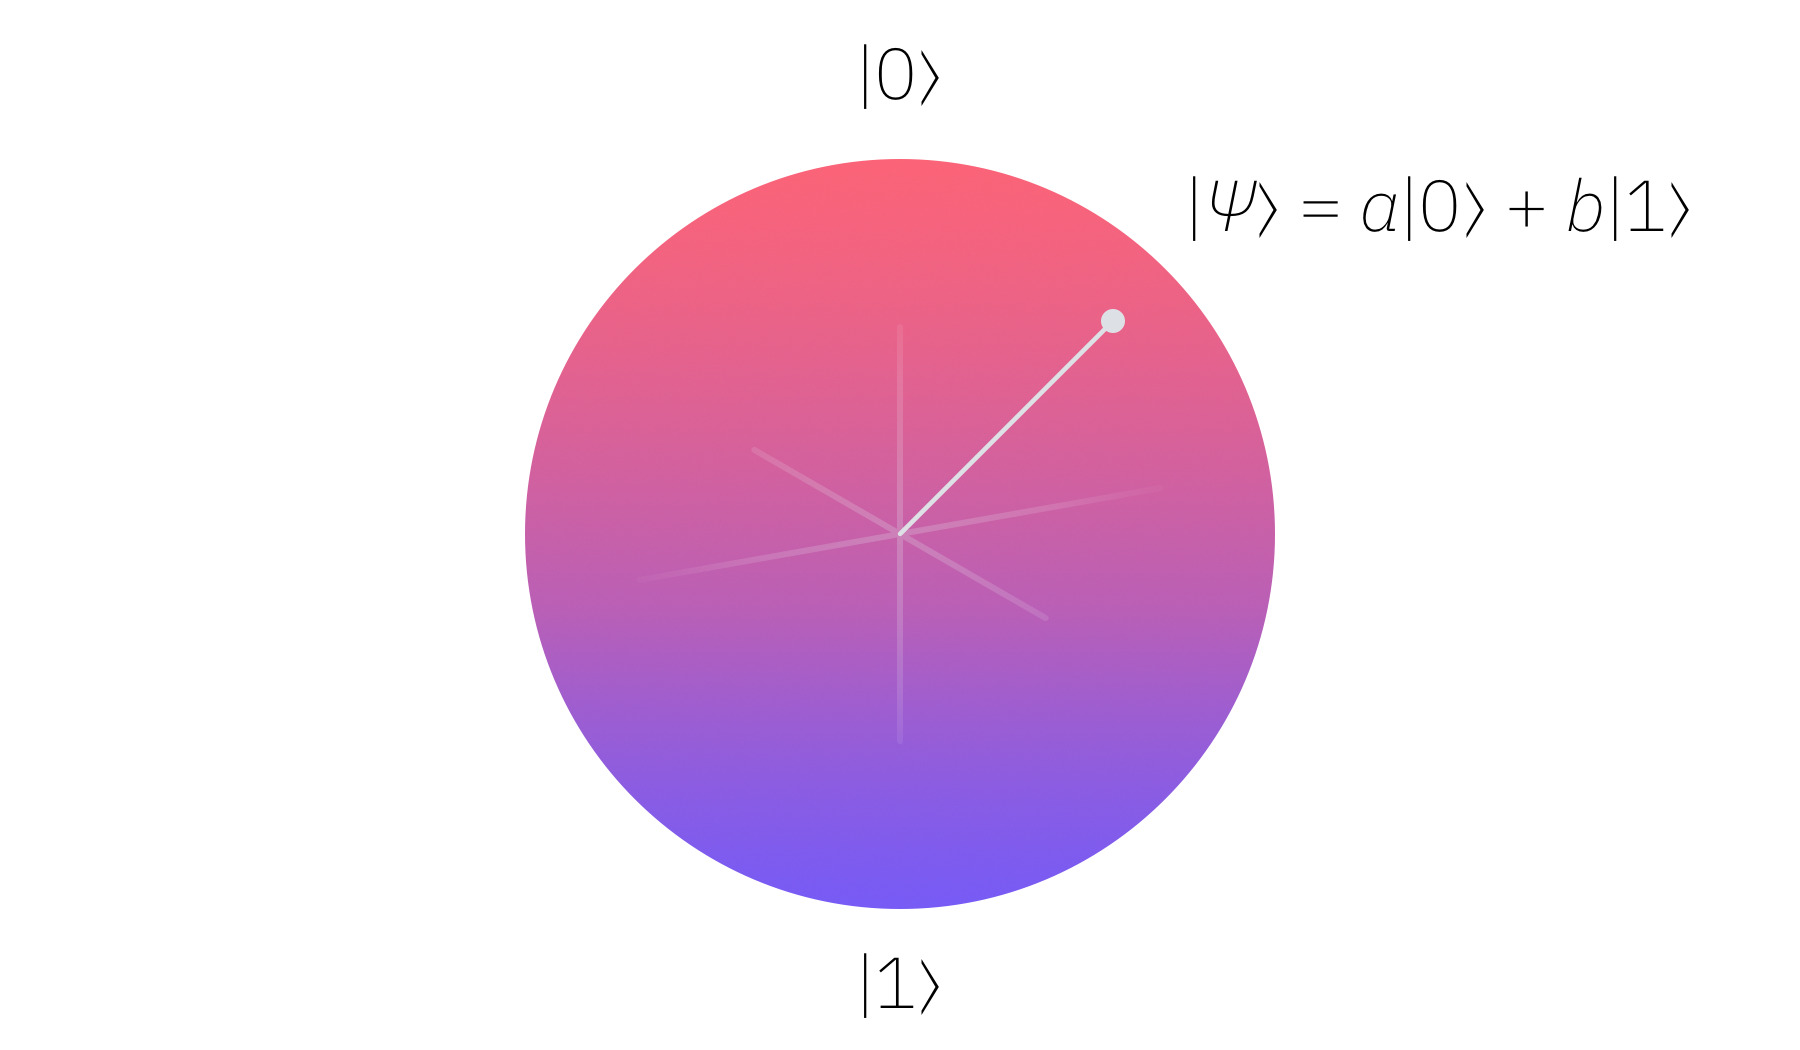
\includegraphics[alt={Testo alternativo dell'immagine}, height=5cm]{img/qubit.jpeg}
    \description[Rappresenzazione Qubit]{Long description}
    \caption{Lorem}
    \label{fig:qubit}
\end{figure}
\lipsum[1]

\section{Processo sviluppo prodotto}
\lipsum[1-2]

\begin{listing}[H]
\begin{minted}{c}
#include <stdio.h>
int main() {
    print("Hello, world!");
    return 0;
}
\end{minted}
\caption{Example of code}
\label{listing:b}
\end{listing}

Lorem ipsum:
\begin{listing}[H]
\begin{minted}{c}
#include <stdio.h>
int main() {
    print("Hello, world!");
    return 0;
}
\end{minted}
\caption{Example of code}
\label{listing:b-2}
\end{listing}

Lorem ipsum:
\begin{listing}[H]
\begin{minted}{c}
#include <stdio.h>
int main() {
    print("Hello, world!");
    return 0;
}
\end{minted}
\caption{Example of code}
\label{listing:b-3}
\end{listing}

\newpage
    \chapter{Descrizione dello stage}
\label{chap:descrizione-stage}

\section{Introduzione al progetto}
\begin{figure}[H] 
    \centering 
    
\includegraphics[alt={Testo alternativo dell'immagine}, width=0.5\columnwidth]{img/pk_estate.jpeg}
    \caption{Caption}
    \label{fig:pk_estate}
\end{figure}
\lipsum[1]

\section{Analisi preventiva dei rischi}

Durante la fase di analisi iniziale sono stati individuati alcuni possibili rischi a cui si potrà andare incontro.
Si è quindi proceduto a elaborare delle possibili soluzioni per far fronte a tali rischi.

\begin{risk}{Performance del simulatore hardware}
    \riskdescription{le performance del simulatore hardware e la comunicazione con questo potrebbero risultare lenti o non abbastanza buoni da causare il fallimento dei test}
    \risksolution{coinvolgimento del responsabile a capo del progetto relativo il simulatore hardware}
    \label{risk:hardware-simulator} 
\end{risk}

\section{Requisiti e obiettivi}

\begin{center}
    \rowcolors{1}{}{tableGray}
    \begin{longtable}{|p{2.25cm}|p{7.75cm}|p{2.25cm}|}
    \hline
    \multicolumn{1}{|c|}{\textbf{A}} & \multicolumn{1}{c|}{\textbf{B}}\\ 
    \hline 
    \endfirsthead
    \rowcolor{white}
    \multicolumn{3}{c}{{\bfseries \tablename\ \thetable{} -- Continuo della tabella}}\\
    \hline
    \multicolumn{1}{|c|}{\textbf{A}} & \multicolumn{1}{c|}{B}\\ \hline 
    \endhead
    \hline
    \rowcolor{white}
    \multicolumn{3}{|r|}{{Continua nella prossima pagina...}}\\
    \hline
    \endfoot
    \endlastfoot 
    
    AA & BB \\
    \hline
    AA & BB \\
    \hline
    AA & BB \\
    \hline
    AA & BB \\
    \hline
    \hiderowcolors
    \caption{Lorem.}
    \label{tab:requisiti_obbiettivi}
    \end{longtable}
\end{center}

\section{Pianificazione}
\begin{figure}[H]
    \centering
    
\includegraphics[alt={Testo alternativo dell'immagine}, width=0.5\columnwidth]{img/pk_estate.jpeg}
    \caption{Caption}
    \label{fig:pk_estate_2}
\end{figure}
\lipsum[1]

\subsection{subsection}
\lipsum[1]

\subsubsection{subsubsection}
\lipsum[1]

\paragraph{paragraph}
\lipsum[1]

\newpage
    \chapter{Analisi dei requisiti}
\label{chap:analisi-requisiti}

\section{Casi d'uso}
Per lo studio dei casi di utilizzo del prodotto sono stati creati dei diagrammi.
I diagrammi dei casi d'uso (in inglese \textit{Use Case Diagram}) sono diagrammi di tipo \gls{uml} dedicati alla descrizione delle funzioni o servizi offerti da un sistema, così come sono percepiti e utilizzati dagli attori che interagiscono col sistema stesso.
Essendo il progetto finalizzato alla creazione di un tool \gls{TermineSenzaAcronimo} per l'automazione di un processo, le interazioni da parte dell'utilizzatore devono essere ovviamente ridotte allo stretto necessario. Per questo motivo i diagrammi d'uso risultano semplici e in numero ridotto.

\begin{figure}[H]
    \vspace{2em}
    \centering
    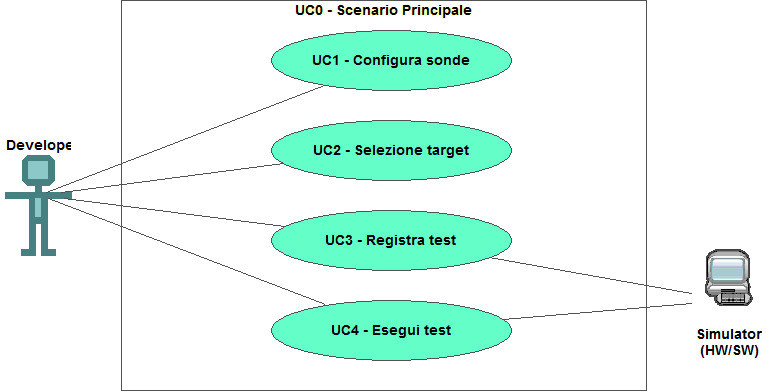
\includegraphics[alt={Testo alternativo dell'immagine}, width=0.75\columnwidth]{img/usecase/scenario-principale.jpeg}
    \caption{Use Case 0: Scenario principale}
    \label{fig:scenario_principale}
\end{figure}

\begin{usecase}{0}{Scenario principale}
    \usecaseactors{Sviluppatore applicativi.}
    \usecasepre{Lo sviluppatore è entrato nel plugin di simulazione all'interno dell'IDE.}
    \usecasedesc{La finestra di simulazione mette a disposizione i comandi per configurare, registrare o eseguire un test.}
    \usecasepost{Il sistema è pronto per permettere una nuova interazione.}
    \label{uc:uc_scenario_principale}
\end{usecase}

\begin{usecase}{1}{Gestione Utente}
    \usecaseactors{Amministratore, Utente Registrato.}
    \usecasepre{L'utente deve essere autenticato nel sistema.}
    \usecasedesc{L'utente può gestire le informazioni del proprio profilo.}
    \usecasepost{Le modifiche vengono salvate nel sistema.}
    \usecasealt{Se l'utente non è autenticato, visualizza un messaggio di errore.}
    \label{uc:uc_casi_uso}
\end{usecase}

\begin{usecase}{2}{Creazione Prodotto}
    \usecaseactors{Amministratore.}
    \usecasepre{L'amministratore ha effettuato l'accesso al sistema.}
    \usecasedesc{L'amministratore può aggiungere un nuovo prodotto al catalogo.}
    \usecasepost{Il nuovo prodotto viene aggiunto con successo.}
    \usecasealt{Se i campi obbligatori non sono compilati, visualizza un messaggio di errore.}
    \label{uc:uc_creazione_prodotto}
\end{usecase}

\section{Tracciamento dei requisiti}
Da un'attenta analisi dei requisiti e degli use case effettuata sul progetto è stata stilata la tabella che traccia i requisiti in rapporto agli use case.\\
Sono stati individuati diversi tipi di requisiti e si è quindi fatto utilizzo di un codice identificativo per distinguerli.\\
Il codice dei requisiti, dove ogni requisito è identificato con il carattere \textbf{R}, è così strutturato:
\begin{enumerate}
    \item[\textbf{F}:] Funzionale.
    \item[\textbf{Q}:] Qualitativo.
    \item[\textbf{V}:] Di vincolo.
    \item[\textbf{N}:] Obbligatorio (necessario).
    \item[\textbf{D}:] Desiderabile.
    \item[\textbf{Z}:] Opzionale.
\end{enumerate}

Nelle tabelle \ref{tab:requisiti_funzionali}, \ref{tab:requisiti_qualitativi} e \ref{tab:requisiti_vincolo} sono riassunti i requisiti e il loro tracciamento con gli use case delineati in fase di analisi.

\section{Tabelle dei requisiti}
\begin{center}
    \rowcolors{1}{}{tableGray}
    \begin{longtable}{|p{2.25cm}|p{7.75cm}|p{2.25cm}|}
    \hline
    %\rowcolor{hyperColor!5}
    \multicolumn{1}{|c|}{\textbf{Requisito}} & \multicolumn{1}{c|}{\textbf{Descrizione}} & \multicolumn{1}{c|}{\textbf{Use Case}}\\
    \hline 
    \endfirsthead
    \rowcolor{white}
    \multicolumn{3}{c}{{\bfseries \tablename\ \thetable{} -- Continuo della tabella}}\\
    \hline
    %\rowcolor{hyperColor!5}
    \multicolumn{1}{|c|}{\textbf{Requisito}} & \multicolumn{1}{c|}{\textbf{Descrizione}} & \multicolumn{1}{c|}{\textbf{Use Case}}\\
    \hline 
    \endhead
    \hline
    \rowcolor{white}
    \multicolumn{3}{|r|}{{Continua nella prossima pagina...}}\\
    \hline
    \endfoot
    \endlastfoot
    
    RFN-1 & L’interfaccia permette di configurare il tipo di sonde del test & UC1 \\
    \hline
    \hiderowcolors
    \caption{Tabella del tracciamento dei requisiti funzionali.}
    \label{tab:requisiti_funzionali}
    \end{longtable}
\end{center}

\begin{center}
    \rowcolors{1}{}{tableGray}
    \begin{longtable}{|p{2.25cm}|p{7.75cm}|p{2.25cm}|}
    \hline
    %\rowcolor{hyperColor!5}
    \multicolumn{1}{|c|}{\textbf{Requisito}} & \multicolumn{1}{c|}{\textbf{Descrizione}} & \multicolumn{1}{c|}{\textbf{Use Case}}\\
    \hline 
    \endfirsthead
    \rowcolor{white}
    \multicolumn{3}{c}{{\bfseries \tablename\ \thetable{} -- Continuo della tabella}}\\
    \hline
    %\rowcolor{hyperColor!5}
    \multicolumn{1}{|c|}{\textbf{Requisito}} & \multicolumn{1}{c|}{\textbf{Descrizione}} & \multicolumn{1}{c|}{\textbf{Use Case}}\\
    \hline 
    \endhead
    \hline
    \rowcolor{white}
    \multicolumn{3}{|r|}{{Continua nella prossima pagina...}}\\
    \hline
    %\caption{Tabella del tracciamento dei requisiti qualitativi.}
    \endfoot
    \endlastfoot
    
    RQD-1n & Le prestazioni del simulatore hardware deve garantire la giusta esecuzione dei test e non la generazione di falsi negativi & - \\
    \hline
    RQD-1n & Le prestazioni del simulatore hardware deve garantire la giusta esecuzione dei test e non la generazione di falsi negativi & - \\
    \hline
    RQD-1n & Le prestazioni del simulatore hardware deve garantire la giusta esecuzione dei test e non la generazione di falsi negativi & - \\
    \hline
    RQD-1n & Le prestazioni del simulatore hardware deve garantire la giusta esecuzione dei test e non la generazione di falsi negativi & - \\
    \hline
    RQD-1n & Le prestazioni del simulatore hardware deve garantire la giusta esecuzione dei test e non la generazione di falsi negativi & - \\
    \hline
    RQD-1n & Le prestazioni del simulatore hardware deve garantire la giusta esecuzione dei test e non la generazione di falsi negativi & - \\
    \hline
    \hiderowcolors
    \caption{Tabella del tracciamento dei requisiti qualitativi.}
    \label{tab:requisiti_qualitativi}
    \end{longtable}
\end{center}

\begin{center}
    \rowcolors{1}{}{tableGray}
    \begin{longtable}{|p{2.25cm}|p{7.75cm}|p{2.25cm}|}
    \hline
    %\rowcolor{hyperColor!5}
    \multicolumn{1}{|c|}{\textbf{Requisito}} & \multicolumn{1}{c|}{\textbf{Descrizione}} & \multicolumn{1}{c|}{\textbf{Use Case}}\\
    \hline 
    \endfirsthead
    \rowcolor{white}
    \multicolumn{3}{c}{{\bfseries \tablename\ \thetable{} -- Continuo della tabella}}\\
    \hline
    %\rowcolor{hyperColor!5}
    \multicolumn{1}{|c|}{\textbf{Requisito}} & \multicolumn{1}{c|}{\textbf{Descrizione}} & \multicolumn{1}{c|}{\textbf{Use Case}}\\
    \hline 
    \endhead
    \hline
    \rowcolor{white}
    \multicolumn{3}{|r|}{{Continua nella prossima pagina...}}\\
    \hline
    \endfoot
    \endlastfoot
    
    RVO-1 & La libreria per l'esecuzione dei test automatici deve essere riutilizzabile & - \\
    \hline
    \hiderowcolors
    \caption{Tabella del tracciamento dei requisiti di vincolo.}
    \label{tab:requisiti_vincolo}
    \end{longtable}
\end{center}

\newpage
    \chapter{Progettazione e codifica}
\label{chap:progettazione-codifica}
Breve introduzione al capitolo

\section{Tecnologie e strumenti}
\label{sec:tecnologie-strumenti}
Di seguito viene data una panoramica delle tecnologie e strumenti utilizzati.

\subsection*{Tecnologia 1}
Descrizione Tecnologia 1.

\subsection*{Tecnologia 2}
Descrizione Tecnologia 2

\section{Ciclo di vita del software}
\label{sec:ciclo-vita-software}

\section{Progettazione}
\label{sec:progettazione}

\subsection{Namespace 1}
Descrizione namespace 1.

\section{Design Pattern utilizzati}

\section{Codifica}
Blocco di codice in C
\begin{listing}[H]
\begin{minted}{c}
#include <stdio.h>
int main() {
    print("Hello, world!");
    return 0;
}
\end{minted}
\caption{Example of code}
\label{listing:c}
\end{listing}

\newpage
    \chapter{Verifica e validazione}
\label{chap:verifica-validazione}

\begin{figure}[H]
    \centering
    
\includegraphics[alt={Testo alternativo dell'immagine}, width=1\columnwidth]{img/quantum_superposition.jpeg}
    \caption{Lorem}
    \label{fig:enter-label}
\end{figure}

\lipsum[1-2]

Lorem ipsum:
\begin{listing}[H]
\begin{minted}{python}
def recur_fibo(n):
   if n <= 1:
       return n
   else:
       return(recur_fibo(n-1) + recur_fibo(n-2))
nterms = 10
if nterms <= 0:
   print("Plese enter a positive integer")
else:
   print("Fibonacci sequence:")
   for i in range(nterms):
       print(recur_fibo(i))
\end{minted}
\caption{Fibonacci recursive}
\label{listing:py_fibo}
\end{listing}

\lipsum[1]

\newpage
    \chapter{Conclusioni}
\label{chap:conclusioni}

\section{Consuntivo finale}
Ipsum

\section{Raggiungimento degli obiettivi}
Sit amet

\section{Conoscenze acquisite}

For applying a subscripting G:\\
Lorem \gls{sdkg}\glox ispum dolor.\\
If the G is followed by a punctuation, such as a "." like in this example, you need to use \textit{gloxspacing}\\
Lorem \gls{sdk}\glox\gloxspacing.\\
Otherwise... \\
Lorem \gls{sdkg}\glox.\\
The "." is not placed in the correct place.\\
Lorem Ipsum dolor \gls{sdkg}\glox\gloxspacing, sit amet.\\
Lorem \gls{apig}

\section{Valutazione personale}
Lorem \gls{umlg}\glox\gloxspacing, ipsum dolor sit amet

\section{Valutazione personale}
Lorem Ipsum dolor Lorem \gls{sdk}

\newpage

    \pagenumbering{roman}
    \backmatter
    \chapter{Bibliografia}
\label{cap:bibliography}

\nocite{*}

% Books bibliography
\printbibliography[heading=subbibliography, title={Testi}, type=book]

% Articles bibliography
\printbibliography[heading=subbibliography, title={Articoli}, type=article]

% Websites bibliography
%\printbibliography[heading=subbibliography, title={Siti}, type=online]

    \chapter{Sitografia}
\label{cap:webliography}
\nocite{*}

% Websites bibliography
\printbibliography[heading=subbibliography, title={\null}, type=online]

\end{document}